\section{Verification}
\label{sec:verification}

This chapter evaluates the performance and learning progression og the Deep Q-network
(DQN)-based pokemon battle agent over two iteration. The objective of this analysis
is to validate the effectiveness of the chosen algorithm and wether we have achieved
the desired results based on our reqirements. Performance is assessed through empirical
training results, including average rewards and win rates.

\subsection{Methodology}
Over the 2 Poke-env iterations, the verification process was conducted using the same hyperparameters
but using different formats of the pokemon battle environment.
The first iteration used a signle battle format with randomly selected pokemon each
episode, while the second iteration was trained using the VGC 2025 regulation G format.
Each version of the agent, was evaluated over a series of training episodes, and data
was collected for:
\begin{itemize}
    \item Average reward per interval of 10 episodes
    \item Win rate per interval of 10 episodes.
\end{itemize}

\subsection{Results and analysis}
\subsubsection{Iteration 1 - Baseline model}
The first iteration exhibited very fluctuating performance, with a relativly shallow
state representation. Although the agent was capable of learning some degree of a control
policy, its reward curve was very erratic and lacked consistency.
\begin{itemize}
    \item The average reward fluctuated significantly, generally ranging between -10 and +5
          indicating the agent struggled to consistently achieve positive outcomes.
    \item Our Agents winrate hovered around 0.4 to 0.6, which isn't generally bad, it's almost a 50\% winrate
          and shows that it performed marginally better with random teams, but still with no clear upward trend.
\end{itemize}
This indicated that while the agent was learning, it was not effectivly generalizing
information across different battle scenarios, largely due to shallow state information.

\begin{figure}[H]
    \centering
    \includegraphics[width=\textwidth]{assets/Iteration-1-graphs.png}
    \caption{Iteration 1 - Baseline model trained over 1000 episodes}
    \label{fig:iteration-1-graphs}
\end{figure}

\subsubsection{Iteration 2 - Enhanced model}
In the second iteration, the agent was restructured to support:
\begin{itemize}
    \item A more complex battle environment.
    \item More modular hyperparameters, allwing for more fine-tunning.
    \item A bigger Q-network, to account for the increased complexity.
\end{itemize}
This meant the improvements to the second iteration resulted in a smoother reward
distribution, altough still noisy, which is typical for reinforcement learning. The variance
is now centered closer to 0, and positive spikes are more frequent. The win rate
had become more stable, despite some episode by episode variation
and was now more consistently above 0.5 with several peaks reacing about 0.8 or 1.0.
Scalablity has also improved significantly. the agent was able to train over 30000 episodes
compared to the just 1000 episodes in the first iteration, without crashing or instability.

Notably, while the average reward trend was still noisy, the longer training horizon
and improved reward shaping, allowed the agent to learn more stable strategies over time.

\begin{figure}[H]
    \centering
    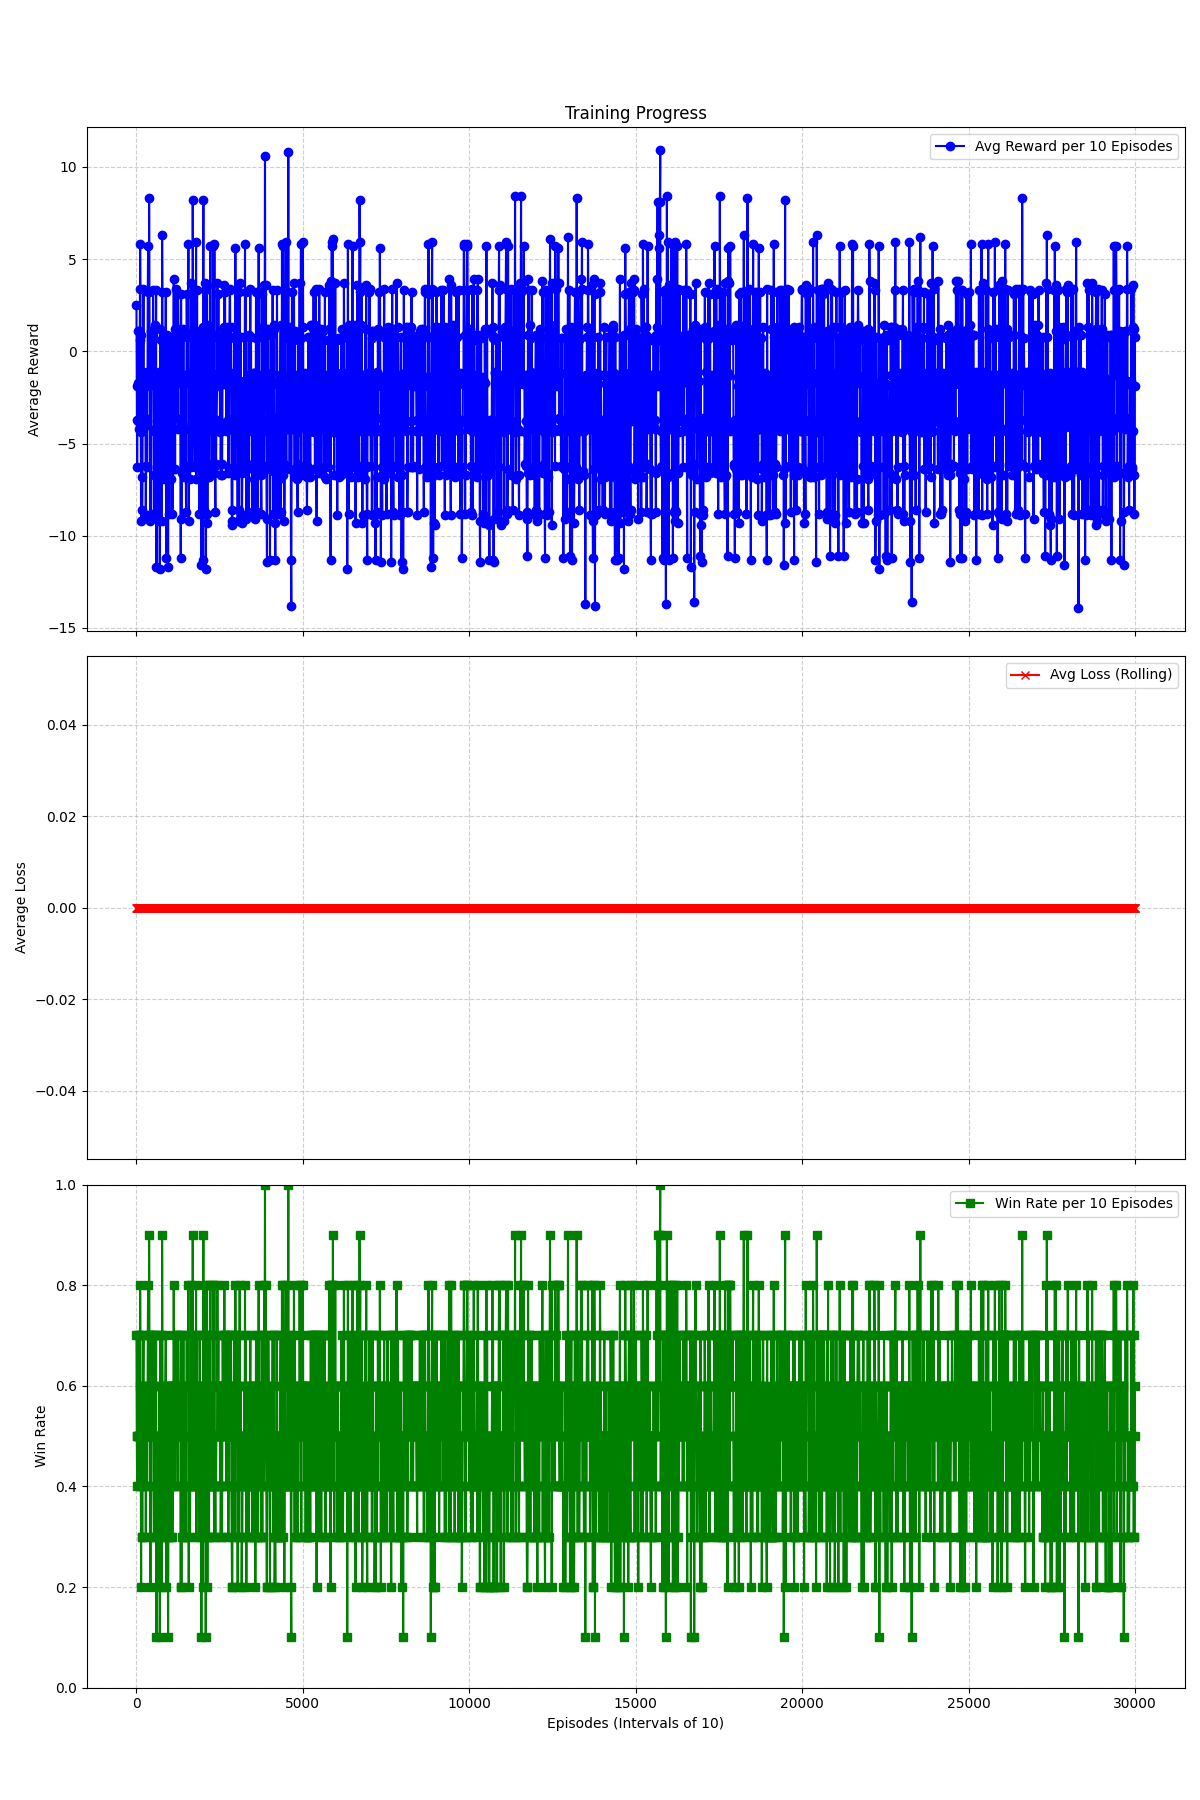
\includegraphics[width=\textwidth]{assets/Iteration-2-graphs.png}
    \caption{Iteration 2 - Enhanced model trained over 30000 episodes}
    \label{fig:iteration-2-graphs}
\end{figure}

\subsubsection{Iteration 3 - Custom environment}

\subsection{Improvements}
The improvements between iterations, can be attributed to several factors:
\begin{itemize}
    \item Expanded state space: Going from a state space of 92 features in the first iteration
          to 128 features in the second iteration, allowed the agent to capture more complex information
          about the environment, leading to better decision making.
    \item Replay buffer: Iteration 2's structured implementation of the replay buffer, improved
          learning consistency and sample efficiency.
    \item Reward design: By incorporating move intermediate rewards (e.g., for defeating enemies or preserving HP),
          the agent receives more meaningful feedback per action, leading to smoother learning curves.
    \item Network Depth: A deeper DQN enabled our model to better capture complex patterns in the data.
\end{itemize}